\documentclass[10pt]{beamer}

\usetheme{Oxygen}
\usepackage{hyperref}
\usepackage[compatibility=false]{caption}
\usepackage{thumbpdf}
\usepackage{wasysym}
\usepackage{ucs}
\usepackage[utf8]{inputenc}
\usepackage{pgf,pgfarrows,pgfnodes,pgfautomata,pgfheaps,pgfshade}
\usepackage{verbatim}
\usepackage{listing}
\usepackage{url}
\usepackage{cite}
\usepackage{minted}

\pdfinfo
{
  /Title       (iOS Application Development)
  /Creator     (TeX)
  /Author      (Chris Zelenak)
}


\title{iOS Application Development}
\subtitle{Day 1}
\author{Chris Zelenak}
\date{06/22/2010}

\begin{document}



\frame{\titlepage}

\section*{}
\begin{frame}
  \frametitle{Outline}
  \tableofcontents[section=1,hidesubsections]
\end{frame}

\AtBeginSection[]
{
  \frame<handout:0>
  {
    \frametitle{Outline}
    \tableofcontents[currentsection,hideallsubsections]
  }
}

\AtBeginSubsection[]
{
  \frame<handout:0>
  {
    \frametitle{Outline}
    \tableofcontents[sectionstyle=show/hide,subsectionstyle=show/shaded/hide]
  }
}

\newcommand<>{\highlighton}[1]{%
  \alt#2{\structure{#1}}{{#1}}
}

\newcommand{\icon}[1]{\pgfimage[height=1em]{#1}}

 

  
    
% BEGIN SECTION Intro to class
\section{Intro to class}
\begin{frame}[fragile]
  \frametitle{Intro to class}
  Welcome to the 4-Day iOS Application Development class. Over the course of these next 4 days, we're going to be reviewing Objective C, UIKit, Core Animation, Core Data, and a host of other technologies you may only know by name.

\end{frame}

\begin{frame}[fragile]
  \frametitle{Intro to class}
  Email me two pictures of you - one serious and one silly - to  chris - at - fastestforward.com

\end{frame}


% END SECTION Intro to class
   
  

  
    
% BEGIN SECTION Lab 1
\section{Lab 1}
\begin{frame}[fragile]
  \frametitle{Lab 1}
  2. Lab 1
\end{frame}


    
\begin{frame}[fragile]
  \frametitle{Create a new iPhone Project}
  Create a new View based application in XCode called Lab1

\end{frame}

\begin{frame}[fragile]
  \frametitle{Create a new iPhone Project}
  Open Lab1ViewController.xib in Interface Builder

\end{frame}

    
\begin{frame}[fragile]
  \frametitle{Add a button}
  Add a button with the text "Hello iPhone"

\end{frame}

    
\begin{frame}[fragile]
  \frametitle{Connect the button to the view controller}
  Add an IBAction selector to the view controller

\end{frame}

\begin{frame}[fragile]
  \frametitle{Connect the button to the view controller}
  Make it open an alert view

\end{frame}

    
\begin{frame}[fragile]
  \frametitle{Build and run in simulator}
  Yay!

\end{frame}

    

% END SECTION Lab 1
   
  

  
    
% BEGIN SECTION Objective C
\section{Objective C}
\begin{frame}[fragile]
  \frametitle{Objective C}
  3. Objective C
\end{frame}


    
\begin{frame}[fragile]
  \frametitle{Overview}
  Objective C is a superset of C. It tacks on to C a message-passing object model similar to Smalltalk's (see Ruby), with a reflective class model built in.

\end{frame}

\begin{frame}[fragile]
  \frametitle{Overview}
  In a more understandable form, Objective C allows you to use weak and dynamicly typed language features along with the static typing of C; it also allows you to take advantage of runtime method resolution, so that your object's implementation of certain messages may be determined at call-time rather than at compile-time.

\end{frame}

\begin{frame}[fragile]
  \frametitle{Overview}
  The language is still physically identical to C in many ways, in that the bulk of your development will be alternating between header files (.h files) and implementation files (.m files). You will also be doing a lot of memory management, which may fill you with either fear or joy, depending on your experience with garbage collected languages.

\end{frame}

\begin{frame}[fragile]
  \frametitle{Overview}
  You will also be dealing a lot with many other C-family familiars, such as enumerated integer constants (enums), structs, pass-by-reference v. pass-by-value semantics and pointers.  You don't need to have a very strong grasp on these things immediately, but the more iPhone programming and Objective C programming you do, the more your skills will benefit from a firm grasp of C.

\end{frame}

    
\begin{frame}[fragile]
  \frametitle{Review of standard C elements}
  These are items you'll commonly encouter while doing iPhone programming whose roots belong in the C family: \begin{listing}[H]
    \begin{minted}[resetmargins=true,fontsize=\footnotesize]{c}
  
  typedef enum {
    NONE = 0,
    SOME,
    ALL
  } ThoseWhoPreferItHot;
  
  ThoseWhoPreferItHot = SOME; // Use of enumerated constant
              
  \end{minted}
    \caption{C Language elements - Enumerations}
    \label{listing:1}
  \end{listing}

\end{frame}

\begin{frame}[fragile]
  \frametitle{Review of standard C elements}
  \begin{listing}[H]
     \begin{minted}[resetmargins=true,fontsize=\footnotesize]{c}
   
   // Declaring a point in space type             
   typedef struct {
     float x;
     float y;
   } APointInSpace;
   
   APointInSpace point;
   point.x = 20.0;
   point.y = 410.0; 
   
   // C99 style struct instantiation              
   APointInSpace point2 = { .x= 21.0, .y=32.0 }; 
              
   \end{minted}
     \caption{C Language Elements - Structs}
     \label{listing:2}
   \end{listing}

\end{frame}

\begin{frame}[fragile]
  \frametitle{Review of standard C elements}
  \begin{listing}[H]
     \begin{minted}[resetmargins=true,fontsize=\footnotesize]{c}
   
   // a constant byte array             
   char * constantCharArray = "Or in other words, a string"; 
   
   // C99 style array instantiation
   int aListOfNumbers[5] = { 1, 2, 3, 4, 5 };
   int aListOfNumbers[] = { 1, 2, 3, 4, 5}; 
   
   // C99 Variable length array declaration
   float aListOfFloats[someQualifier];
   
   // pointer declaration to NULL              
   int * someIntegerPtr = NULL; 
   int someInteger = 5;
   
   // address dereference              
   someIntegerPtr = &someInteger; 
               
   \end{minted}
     \caption{C Language Elements - Arrays and Pointers}
     \label{listing:3}
   \end{listing}

\end{frame}

\begin{frame}[fragile]
  \frametitle{Review of standard C elements}
  If you've not kept abreast of changes between ANSI-92 C (a common version of C taught in universities and in many books about C) and C99, read more at \url{http://home.datacomm.ch/t_wolf/tw/c/c9x_changes.html} \cite{C99Changes}.

\end{frame}

    
\begin{frame}[fragile]
  \frametitle{Syntax}
  \begin{listing}[H]
    \begin{minted}[resetmargins=true,fontsize=\footnotesize]{objectivec}
  
  NSString * anExampleString = @"This is a pointer to an NSString object";
  int strLen = [anExampleString length];
             
  NSString * aSecondString = [anExampleString
    stringByAppendingString:@" that had a second string appended to it"];
            
  if([anExampleString
       compare:@"this is a pointer to an nsstring object"
       options:NSCaseInsensitiveCompare] == NSOrderedSame){
    NSLog(@"The string %@ was case insensitive equal", anExampleString);
  }
            
  \end{minted}
    \caption{Some typical Objective C code}
    \label{listing:4}
  \end{listing}

\end{frame}

    
\begin{frame}[fragile]
  \frametitle{Calling functions}
  Given some Objective C object, like:
\begin{minted}[resetmargins=true,fontsize=\footnotesize]{objectivec}
  
  NSString * anObject = @"TheObject";
            
  \end{minted}

you can invoke functionality on that object via the form:
\begin{minted}[resetmargins=true,fontsize=\footnotesize]{objectivec}
 
 [anObject theMethodName];
           
 \end{minted}

Method names in Objective C follow the form initialMethodNameAndArgument:theSecondArgument:theThirdArgument: . 
\begin{block}{Messages vs. Methods}
  
  When you see references to "calling a method" or "calling a function" on an object in Objective C, it's best to
  consider these synonymous with "dispatching a message".  Objective C objects respond to
  \highlighton{messages}, and as you work more with Objective C, it will be more beneficial for
  you to perceive this as such.  
            
  \end{block}

\end{frame}

    
\begin{frame}[fragile]
  \frametitle{nil, NULL}
  An object in Objective C may be nil; nil is a "special" object which may have any message at all sent to it, to which it will respond with a nil object.
\begin{listing}[H]
    \begin{minted}[resetmargins=true,fontsize=\footnotesize]{objectivec}
  
  NSString * anObject = nil;
  if([anObject whoaThisProbablyDoesntExist] == nil){
    NSLog(@"Ah well");
  }
            
  \end{minted}
    \caption{nil object responding to any message}
    \label{listing:5}
  \end{listing}

nil is the appropriate null object when dealing with pointers to Objective C classes; NULL, on the other hand, is the appropriate null value to use when dealing with pointers to all other types.

\end{frame}

    
\begin{frame}[fragile]
  \frametitle{Classes}
  
\end{frame}

    
\begin{frame}[fragile]
  \frametitle{Memory management}
  Objective C's memory management model is a reference counting system that you can think of as an integer counter assigned to each object. Each object, when initialized, starts with a counter equal to 1.  When this counter reaches 0, the cleanup functions (dealloc) on the object are called and the memory for the object is released back to the system.

\end{frame}

\begin{frame}[fragile]
  \frametitle{Memory management}
  \begin{listing}[H]
    \begin{minted}[resetmargins=true,fontsize=\footnotesize]{objectivec}
  
  // Retain count of 1            
  NSString * foo = [[NSString alloc] initWithString:@"Foo"]; 
  [foo retain]; // Retain count of 2
  NSLog(@"Foo is %@", foo);
  [foo release]; // Retain count of 1
  NSLog(@"Foo is still %@", foo);
  [foo release]; // Retain count of 0,
                 // foo is released back to the system
                 
  // This will crash the program (EXC_BAD_ACCESS)
  NSLog(@"Foo crashes %@", foo); 
              
  \end{minted}
    \caption{Memory management in Objective C}
    \label{listing:9}
  \end{listing}
\begin{block}{EXC BAD ACCESS ? What?}
  
  EXC BAD ACCESS is the error message your program will output when
  it attempts to do something to a pointer to a memory location
  whose contents have previously been released to the system.
              
  \end{block}

\end{frame}

\begin{frame}[fragile]
  \frametitle{Memory management}
  You can indicate you don't want to manage the release of an object by indicating an object should be autoreleased objects.  Autoreleased objects are managed by an object called an NSAutoreleasePool, and are intermittently checked to see how many references have been claimed on them.  The pool will release the object "at some unknown point in the future"* once all  retains on the object have been released.

\end{frame}

\begin{frame}[fragile]
  \frametitle{Memory management}
  \begin{listing}[H]
    \begin{minted}[resetmargins=true,fontsize=\footnotesize]{objectivec}
  
  // Indicate that the foo object should be managed by
  // the current NSAutoreleasePool
  NSString * foo = [[[NSString alloc]
                               initWithString:@"Foo"]
                                 autorelease];
  NSLog(@"Foo will be good for now %@", foo);
  
  [foo retain]; 
  [foo release];
  NSLog(@"Foo is still good, %@", foo);
  // You may retain and release on an autoreleased object as normal
  
  [foo release];
  // Calling an 'unbalanced release' like this will cause a crash
  // at some unknown point in the future
              
  \end{minted}
    \caption{Memory management in Objective C}
    \label{listing:10}
  \end{listing}

\end{frame}

\begin{frame}[fragile]
  \frametitle{Memory management}
  Different classes in Cocoa / Objective C have different rules about how they retain objects.  The documentation is instructive in telling you what memory management semantics you should expect from given functionality.
\begin{block}{Mac Programmers Have All The Luck}
  
  Should you be programming Mac OS applications as opposed to iOS applications,
  you can take advantage of garbage collection memory management which has been
  available since Mac OS Leopard (10.5); iOS programmers still have to manage their
  memory themselves, however.
              
  \end{block}

\end{frame}

    
\begin{frame}[fragile]
  \frametitle{Properties}
  Much of the interaction with Objective C objects equates to the usual getter/setter functionality commonly associated with Object Oriented Programming. To make it easier for programmers to declare this functionality, properties were introduced as a way to eschew all the boilerplate code and provide a common framework upon which to enhance Objective C objects.

\end{frame}

\begin{frame}[fragile]
  \frametitle{Properties}
  \begin{listing}[H]
    \begin{minted}[resetmargins=true,fontsize=\footnotesize]{objectivec}
  
  @interface MyObject : NSObject {
    NSString * instanceVariable;
    float numericVariable;
  }
  @property(readwrite, retain) NSString * instanceVariable;
  @property(readonly, assign) float numericVariable;
  @end
  
  @implementation MyObject
  
  @synthesize instanceVariable;
  @synthesize numericVariable;
  
  -(void) dealloc {
    [instanceVariable release];
    [super dealloc];
  }
  
  @end 
    
              
  \end{minted}
    \caption{Property interface declaration}
    \label{listing:11}
  \end{listing}

\end{frame}

\begin{frame}[fragile]
  \frametitle{Properties}
  \begin{listing}[H]
    \begin{minted}[resetmargins=true,fontsize=\footnotesize]{objectivec}
  
  MyObject * mo = [[MyObject alloc] init];
  [mo setInstanceVariable:@"Test"];
  [mo setNumericVariable:20.0f];
  NSLog(@"The values I set were %@ and %f",
          [mo instanceVariable], 
          [mo numericVariable]);
              
  \end{minted}
    \caption{Property usage}
    \label{listing:12}
  \end{listing}

\end{frame}

\begin{frame}[fragile]
  \frametitle{Properties}
  You can specify the memory management semantics (retain, assign, copy) in the property declaration.  You can also specify the atomicity (locking behavior) of the property, and more.
\begin{block}{More to it..}
  
  Properties do not merely provide getter/setter functionality.  The use of properties
  also implicitly adds Key-Value-Observing functionality to your class, letting
  you automatically monitor classes for change events and performing specific code
  in such cases.  Read more at \url{http://developer.apple.com/mac/library/documentation/cocoa/conceptual/objectivec/articles/ocProperties.html}.
              
  \end{block}

\end{frame}

    
\begin{frame}[fragile]
  \frametitle{Selectors}
  Selectors in Objective C are a way to provide a special type to indicate a message. They allow you to dynamically send a message to an object, as well as to query an object to see if it responds to a given message.

\end{frame}

\begin{frame}[fragile]
  \frametitle{Selectors}
  \begin{listing}[H]
    \begin{minted}[resetmargins=true,fontsize=\footnotesize]{objectivec}
  
  SEL aSelector = @selector(length);
  NSString * foo = @"Foo";
  if([foo respondsToSelector:aSelector]){
    NSLog(@"The length of foo is %i",  [foo performSelector:aSelector]);
  }
  
              
  \end{minted}
    \caption{Selector usage}
    \label{listing:13}
  \end{listing}

\end{frame}

\begin{frame}[fragile]
  \frametitle{Selectors}
  Selectors can be built from strings, and can refer to any Objective C message that is forwarded to an object. \begin{listing}[H]
    \begin{minted}[resetmargins=true,fontsize=\footnotesize]{objectivec}
  
  NSString * aUserSuppliedString = MagicallyGetStringFromUserInput();
  SEL aSelector = NSSelectorFromString(aUserSuppliedString);
  if([someObject respondsToSelector:aSelector]){
    // NOTE: Surely nothing bad will happen
    [someObject performSelector:aSelector];
  }
              
  \end{minted}
    \caption{Other selector usage}
    \label{listing:14}
  \end{listing}

\end{frame}

    
\begin{frame}[fragile]
  \frametitle{Protocols}
  Objective C provides only single-inheritance for its objects; to allow for situations where a class may provide functionality outside of its inheritance chain, the language provides Protocols, which are roughly analogous to interfaces in Java and C\#.  There are informal protocols (only referred to in documentation) and formal protocols, which are compiler checked.  The majority of protocol usage in iOS programming is formal protocols.

\end{frame}

\begin{frame}[fragile]
  \frametitle{Protocols}
  \begin{listing}[H]
    \begin{minted}[resetmargins=true,fontsize=\footnotesize]{objectivec}
  
  @protocol TestProtocol
  
  -(void) definitelyHasThisMethod;
  
  @optional
  
  -(void) mayHaveThisMethod;
  
  @end
              
  \end{minted}
    \caption{Protocol declaration}
    \label{listing:15}
  \end{listing}
\begin{listing}[H]
  \begin{minted}[resetmargins=true,fontsize=\footnotesize]{objectivec}

@interface SomeObject : NSObject<TestProtocol> {
}
@end 
\end{minted}
  \caption{Protocol conformance}
  \label{listing:16}
\end{listing}

\end{frame}

\begin{frame}[fragile]
  \frametitle{Protocols}
  \begin{listing}[H]
    \begin{minted}[resetmargins=true,fontsize=\footnotesize]{objectivec}
  
  SomeObject<TestProtocol> * oo = [[SomeObject alloc] init];
  
  // We assume this because the object conforms to TestProtocol              
  [oo definitelyHasThisMethod];
  
  if([oo respondsToSelector:@selector(mayHaveThisMethod)]){
    [oo mayHaveThisMethod];
  }
              
  \end{minted}
    \caption{Protocol usage}
    \label{listing:17}
  \end{listing}

\end{frame}

    
\begin{frame}[fragile]
  \frametitle{Categories}
  Categories allow you to mix in new code to existing classes without having to change the original source code for those classes.  Examples of categories include automatically adding special serialization rules to NSObject, or special data structure Queue behavior to Cocoa collection classes.
\begin{alertblock}{Except for..}
  
  You can't add instance variables to a class with categories; they are
  purely for adding new methods to a class, but cannot change the memory
  layout of a class after the fact.
              
  \end{alertblock}

\end{frame}

\begin{frame}[fragile]
  \frametitle{Categories}
  \begin{listing}[H]
    \begin{minted}[resetmargins=true,fontsize=\footnotesize]{objectivec}
  
  @interface NSString(FunkyStrings)
  
  -(NSString *) getFunky;
  
  @end
  
  @implementation NSString(FunkyStrings)
  
  -(NSString *) getFunky {
    return [self stringByAppendingString:@"...YEAH! ALL RIGHT! FEELS GOOD!"];
  }
  
  @end
              
  \end{minted}
    \caption{Category declaration}
    \label{listing:18}
  \end{listing}

\end{frame}

\begin{frame}[fragile]
  \frametitle{Categories}
  \begin{listing}[H]
  \begin{minted}[resetmargins=true,fontsize=\footnotesize]{objectivec}

#import "NSString+FunkyStrings.h"
void main(){
  NSLog(@"The funkiest string by far is %@", [@"James Brown" getFunky]);
}
\end{minted}
  \caption{Category usage}
  \label{listing:19}
\end{listing}

\end{frame}

    
\begin{frame}[fragile]
  \frametitle{Review common useful classes in Objective C / Cocoa to accomplish certain tasks}
  There are a host of useful classes in the Cocoa Touch framework that provide special functionality to you.  Some of the more common objects you'll use in your programming are NSArray, NSDictionary, NSNumber and NSString.  Each of these objects have mutable versions that allow you to modify them after instantiation.

\end{frame}

\begin{frame}[fragile]
  \frametitle{Review common useful classes in Objective C / Cocoa to accomplish certain tasks}
  NSString is an enhanced, unicode aware string class that goes far beyond the simple byte-array behavior of C's byte-array strings.
\begin{listing}[H]
    \begin{minted}[resetmargins=true,fontsize=\footnotesize]{objectivec}
  
  NSString * s = [[NSString alloc] initWithCString:"this is an ascii string"
                                   encoding:NSASCIIStringEncoding];
  NSMutableString * so = [[NSMutableString alloc]
                                  initWithString:@"A mutable string with..."];
  
  [so appendString:s];
  
  NSLog(@"The mutable string is %@", so);
  
  [so release];
  [s release];
              
  \end{minted}
    \caption{NSString usage}
    \label{listing:20}
  \end{listing}

\end{frame}

\begin{frame}[fragile]
  \frametitle{Review common useful classes in Objective C / Cocoa to accomplish certain tasks}
  NSNumber is a simple abstract wrapper around numeric values which allows you to automatically convert its held value to the appropriate form, as well as having an object-like representations of a numeric value.
\begin{listing}[H]
    \begin{minted}[resetmargins=true,fontsize=\footnotesize]{objectivec}
  
  NSNumber * n = [[NSNumber alloc] initWithFloat:20.0f];
  double d = [n doubleValue];
  int i = [n intValue];
  [n release];
              
  \end{minted}
    \caption{NSNumber usage}
    \label{listing:21}
  \end{listing}

\end{frame}

\begin{frame}[fragile]
  \frametitle{Review common useful classes in Objective C / Cocoa to accomplish certain tasks}
  NSDictionary is a generic dictionary object that you can use to hold key/value associations. A key can be any NSObject that responds to isEqual: and NSCopying; in most cases, your keys will be either NSString or NSNumber objects.

\end{frame}

\begin{frame}[fragile]
  \frametitle{Review common useful classes in Objective C / Cocoa to accomplish certain tasks}
  \begin{listing}[H]
    \begin{minted}[resetmargins=true,fontsize=\footnotesize]{objectivec}
  
  NSDictionary * a = [[NSDictionary alloc] initWithObjectsAndKeys:
                                        @"The foo string", @"Foo",
                                        @"The bar string", @"Bar",
                                        nil];
  
  NSMutableDictionary * b = [[NSMutableDictionary alloc] init];
  [b setObject:@"Another string" forKey:[NSNumber numberWithInt:20]];
  
  NSLog(@"a's alue for Foo is %@, and b's value for 20 is %@",
                            [a objectForKey:@"Foo"],
                            [b objectForKey:[NSNumber numberWithInt:20]]);
  
  for(id key in a){
    NSLog(@"The value for %@ is %@", key, [a objectForKey:key]);
  }
  
  [b release];
  [a release];
              
  \end{minted}
    \caption{NSDictionary usage}
    \label{listing:22}
  \end{listing}

\end{frame}

\begin{frame}[fragile]
  \frametitle{Review common useful classes in Objective C / Cocoa to accomplish certain tasks}
  NSArray is a simple way to collect NSObject inheriting classes into a sequential list.  NSArray automatically retains each object added to it, and releases each object it holds once its own retain count has reached 0.
\begin{listing}[H]
    \begin{minted}[resetmargins=true,fontsize=\footnotesize]{objectivec}
  
  NSArray * a = [[NSArray alloc] initWithObjects:@"Foo", @"bar", @"baz", nil];
  NSMutableArray * b = [[NSMutableArray alloc] init];
  [b addObject:@"Not foo"];
  NSLog(@"The contents of a are %@ and b are %@", a, b);
  
  for(NSString * obj in a){
    NSLog(@"The array contains %@", obj);
  }
  
  [a release];
  [b release];
              
  \end{minted}
    \caption{NSArray usage}
    \label{listing:23}
  \end{listing}

\end{frame}

\begin{frame}[fragile]
  \frametitle{Review common useful classes in Objective C / Cocoa to accomplish certain tasks}
  NSArray, NSDictionary, NSString and NSNumber may all be represented by the contents of a property list file ( Plist ).  You can easily rebuild an NSArray or NSDictionary full of the property list contents by using the initialization method \highlighton{initWithContentsOfFile:}

\end{frame}

\begin{frame}[fragile]
  \frametitle{Review common useful classes in Objective C / Cocoa to accomplish certain tasks}
  \begin{figure}[htb]
  \begin{center}
  
  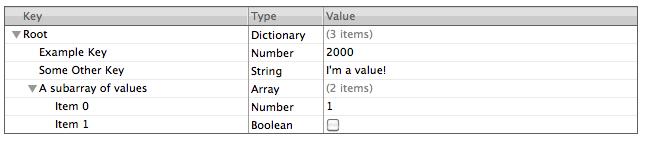
\includegraphics[scale=0.5]{PListExample1.png}
              
  \caption{Sample Property List}
  \end{center}
  \end{figure}

\begin{listing}[H]
    \begin{minted}[resetmargins=true,fontsize=\footnotesize]{objectivec}
  
  NSDictionary * example = [[NSDictionary alloc]
                               initWithContentsOfFile:@"/path/to/sample.plist"];
  NSLog(@"The subarray contents are %@",
             [example objectForKey:"A subarray of values"]);
  [example release];
              
  \end{minted}
    \caption{Property List Deserialization}
    \label{listing:24}
  \end{listing}

\end{frame}

    
\begin{frame}[fragile]
  \frametitle{More learning}
  Objective C is a rich, deep language.  There are lots of resources on the web and your computer where you can learn more. The best is easily the XCode documentation, but there are blogs out there that can provide invaluable help: Mike Ash's NSBlog \url{http://www.mikeash.com/pyblog/},  Cocoa With Love \url{http://cocoawithlove.com/}, and the Apple Developer Forums \url{http://developer.apple.com/devforums/} can all provide invaluable help in learning new techniques and advanced usage for your apps.

\end{frame}

    

% END SECTION Objective C
   
  

  
    
% BEGIN SECTION iPhone App Layout Conventions
\section{iPhone App Layout Conventions}
\begin{frame}[fragile]
  \frametitle{iPhone App Layout Conventions}
  4. iPhone App Layout Conventions
\end{frame}


    
\begin{frame}[fragile]
  \frametitle{MVC, as applied to an app}
  Apple strongly encourages you to adhere to Model View Controller pattern

\end{frame}

    
\begin{frame}[fragile]
  \frametitle{Application -> Window -> View Controller(s) -> View(s) + Models}
  On iOS, a UIApplication ( your app ) typically has one UIWindow, which is the primary UIView upon which everything else displays.  A UIView is just a rectangle upon which you draw things.

\end{frame}

\begin{frame}[fragile]
  \frametitle{Application -> Window -> View Controller(s) -> View(s) + Models}
  Almost everything visual is a UIView (except the things that aren't).

\end{frame}

\begin{frame}[fragile]
  \frametitle{Application -> Window -> View Controller(s) -> View(s) + Models}
  \begin{figure}[htb]
  \begin{center}
  
  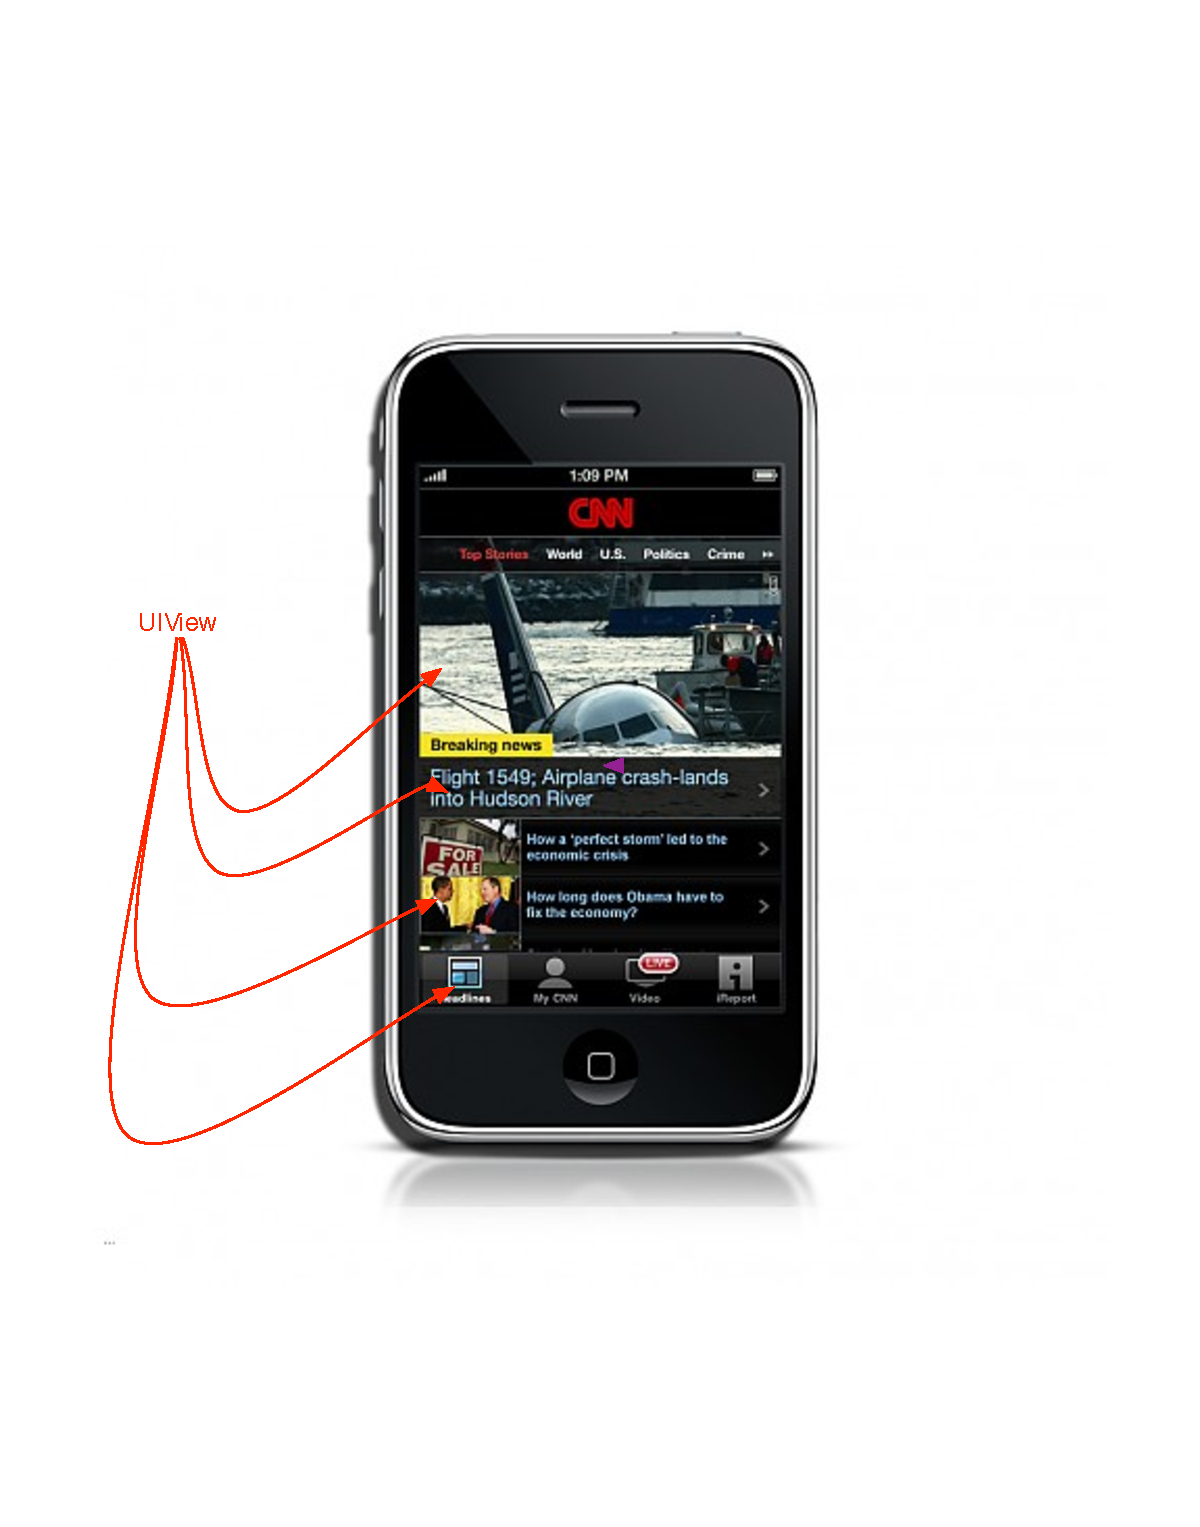
\includegraphics[scale=0.35]{UIViewExample.pdf}
              
  \caption{UIViews are everything}
  \end{center}
  \end{figure}

\end{frame}

\begin{frame}[fragile]
  \frametitle{Application -> Window -> View Controller(s) -> View(s) + Models}
  \begin{figure}[htb]
  \begin{center}
  
  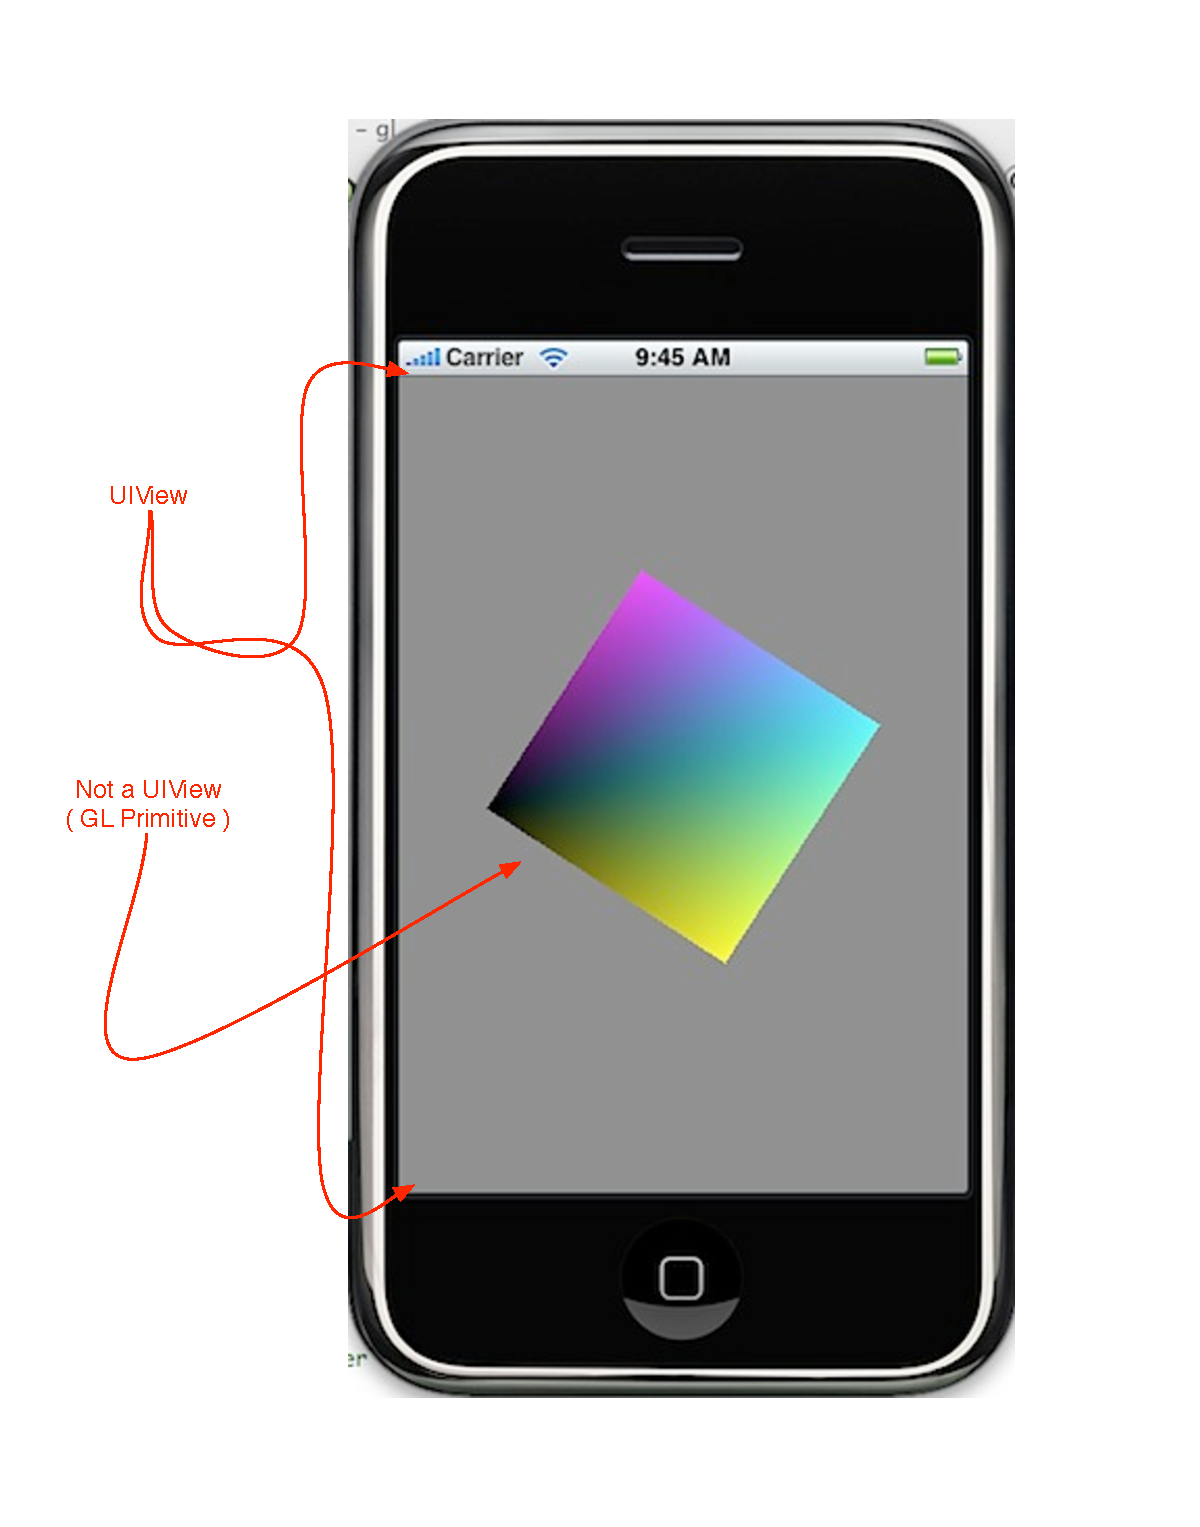
\includegraphics[scale=0.35]{UIViewExample2.pdf}
              
  \caption{UIViews are almost everythign}
  \end{center}
  \end{figure}

\end{frame}

\begin{frame}[fragile]
  \frametitle{Application -> Window -> View Controller(s) -> View(s) + Models}
  UIViewControllers are objects that manage what the views on screen are currently doing; typically where you write event handling code and user interaction code.

\end{frame}

\begin{frame}[fragile]
  \frametitle{Application -> Window -> View Controller(s) -> View(s) + Models}
  You provide the model

\end{frame}

    
\begin{frame}[fragile]
  \frametitle{UINavigationController}
  UINavigationController is a stack based manager of view controllers that the user can navigate through

\end{frame}

\begin{frame}[fragile]
  \frametitle{UINavigationController}
  \begin{figure}[htb]
  \begin{center}
  
  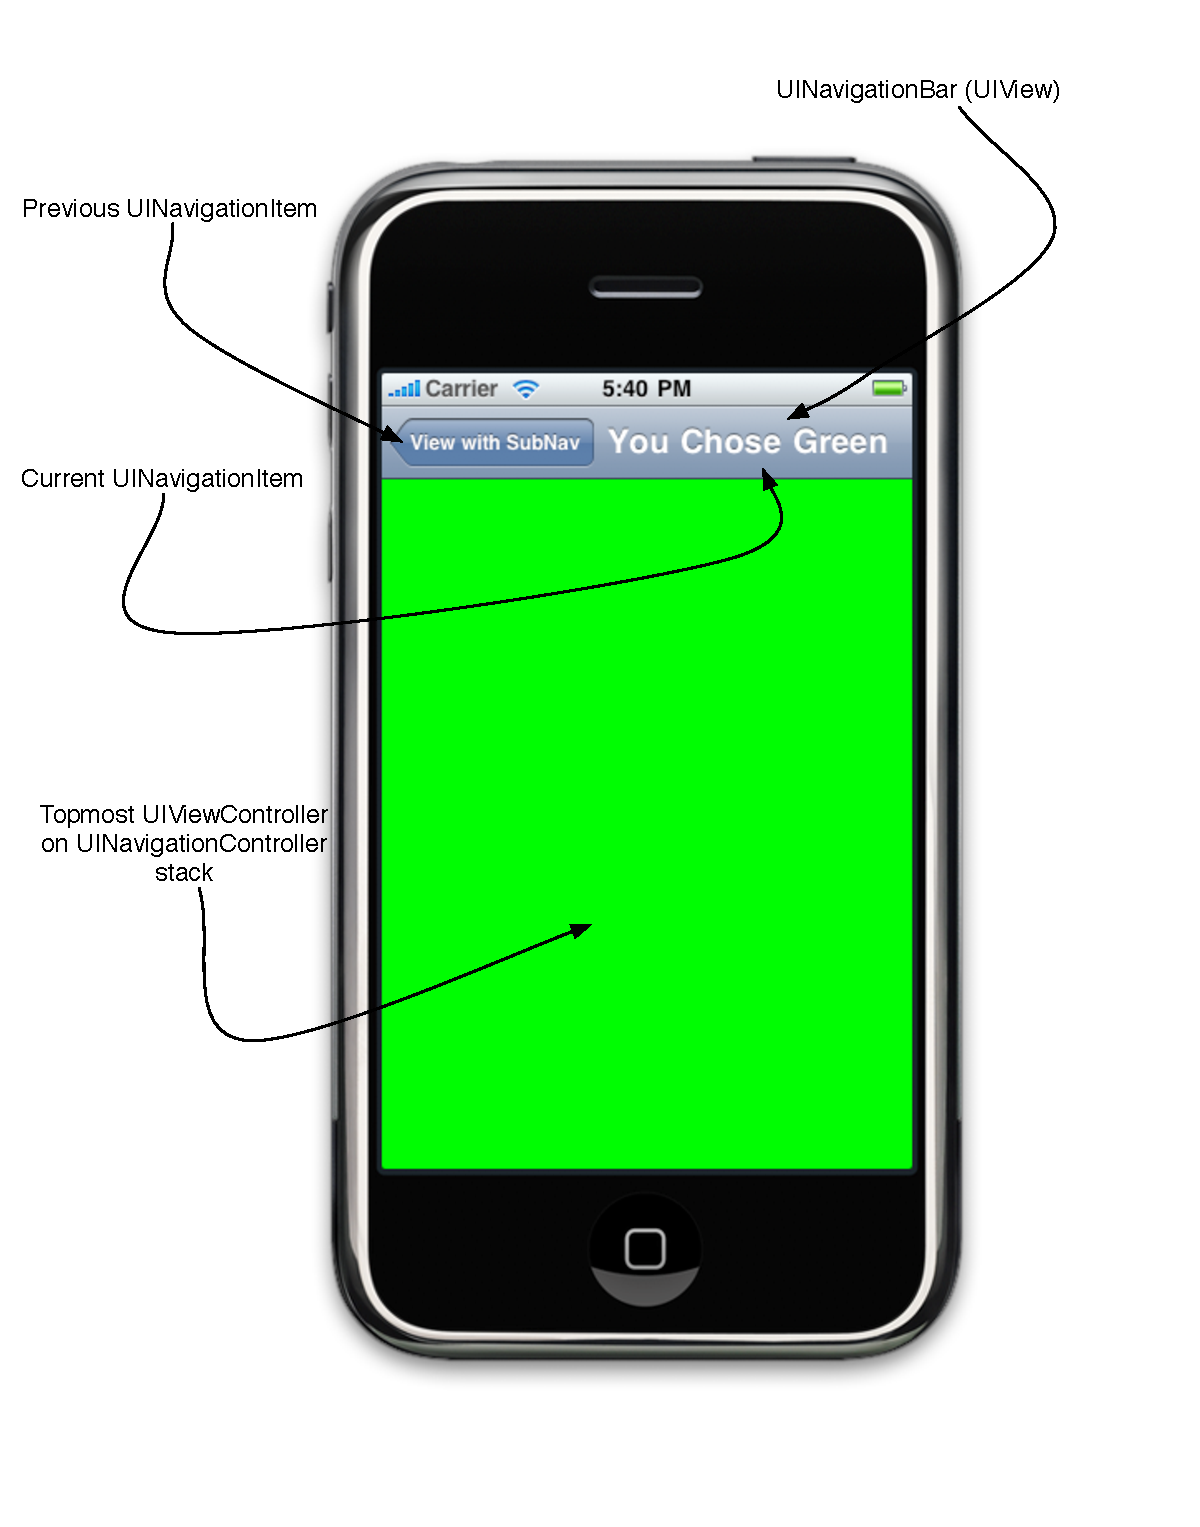
\includegraphics[scale=0.35]{UIViewExample3.pdf}
              
  \caption{Items managed by UINavigationController }
  \end{center}
  \end{figure}

\end{frame}

\begin{frame}[fragile]
  \frametitle{UINavigationController}
  Every UIViewController managed by a UINavigationController has a reference to that UINavigationController

\end{frame}

\begin{frame}[fragile]
  \frametitle{UINavigationController}
  \begin{listing}[H]
    \begin{minted}[resetmargins=true,fontsize=\footnotesize]{objectivec}
  
  MyViewController * controller = [[MyViewController alloc] initWithNibName:nil
                                                            bundle:nil];
  [[self navigationController] pushViewController:controller animated:YES];
  [controller release];
              
  \end{minted}
    \caption{Adding another UIViewController to the UINavigationController stack}
    \label{listing:25}
  \end{listing}

\end{frame}

    
\begin{frame}[fragile]
  \frametitle{Lab 2}
  Create a new View based project

\end{frame}

\begin{frame}[fragile]
  \frametitle{Lab 2}
  Add a UINavigationController to MainWindow.xib

\end{frame}

\begin{frame}[fragile]
  \frametitle{Lab 2}
  Create a new view controller

\end{frame}

\begin{frame}[fragile]
  \frametitle{Lab 2}
  Add a button to the first view controller and create an action to open the second view controller

\end{frame}

    
\begin{frame}[fragile]
  \frametitle{UITabBarController and UITableViewController}
  UITabBarController swaps in UIViewControllers assigned to it when users click on the associated button

\end{frame}

\begin{frame}[fragile]
  \frametitle{UITabBarController and UITableViewController}
  Each UIViewController has a tabBarItem property that UITabBarController uses to populate its UITabBar

\end{frame}

\begin{frame}[fragile]
  \frametitle{UITabBarController and UITableViewController}
  \begin{figure}[htb]
  \begin{center}
  
  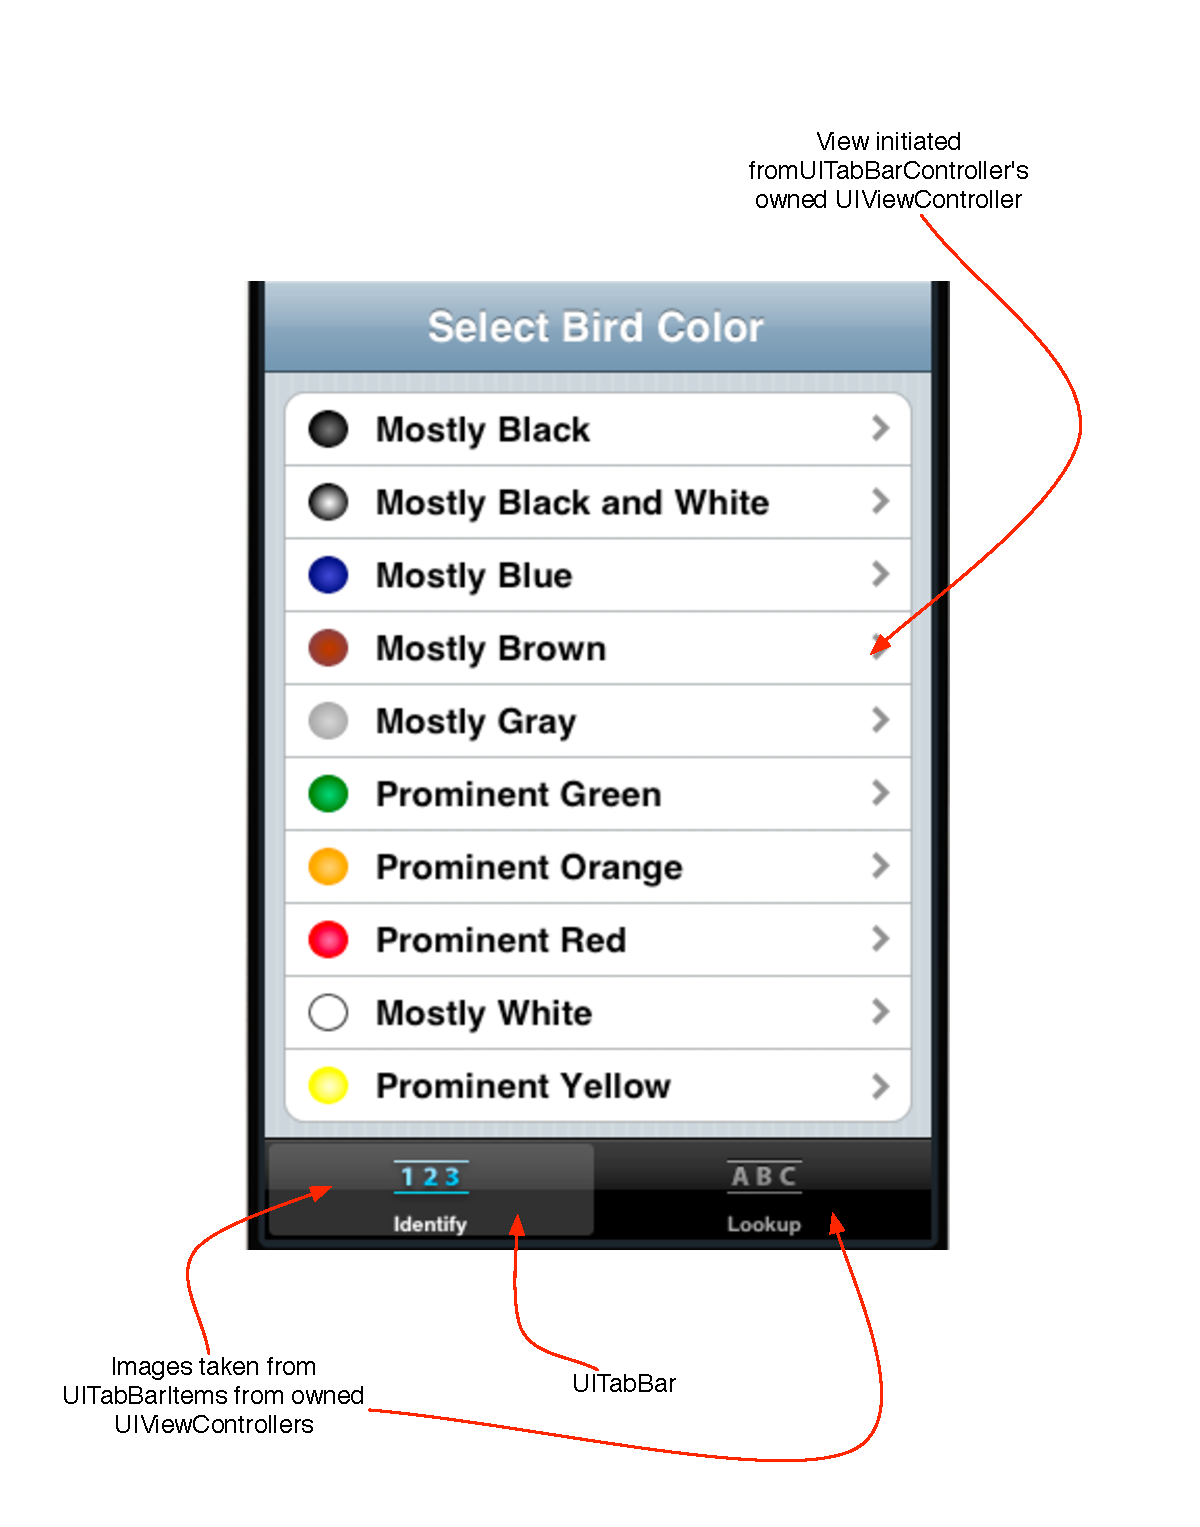
\includegraphics[scale=0.3]{UIViewExample4.pdf}
              
  \caption{UITabBarController example}
  \end{center}
  \end{figure}

\end{frame}

\begin{frame}[fragile]
  \frametitle{UITabBarController and UITableViewController}
  UITableViewController instructs a UITableView about the number of rows it contains, what to do when clicked, the number of sections, and other information

\end{frame}

\begin{frame}[fragile]
  \frametitle{UITabBarController and UITableViewController}
  UITableViewController is just a convenience class that saves you from manually conforming an object to the UITableViewDataSource and UITableViewDelegate protocols

\end{frame}

\begin{frame}[fragile]
  \frametitle{UITabBarController and UITableViewController}
  \begin{figure}[htb]
  \begin{center}
  
  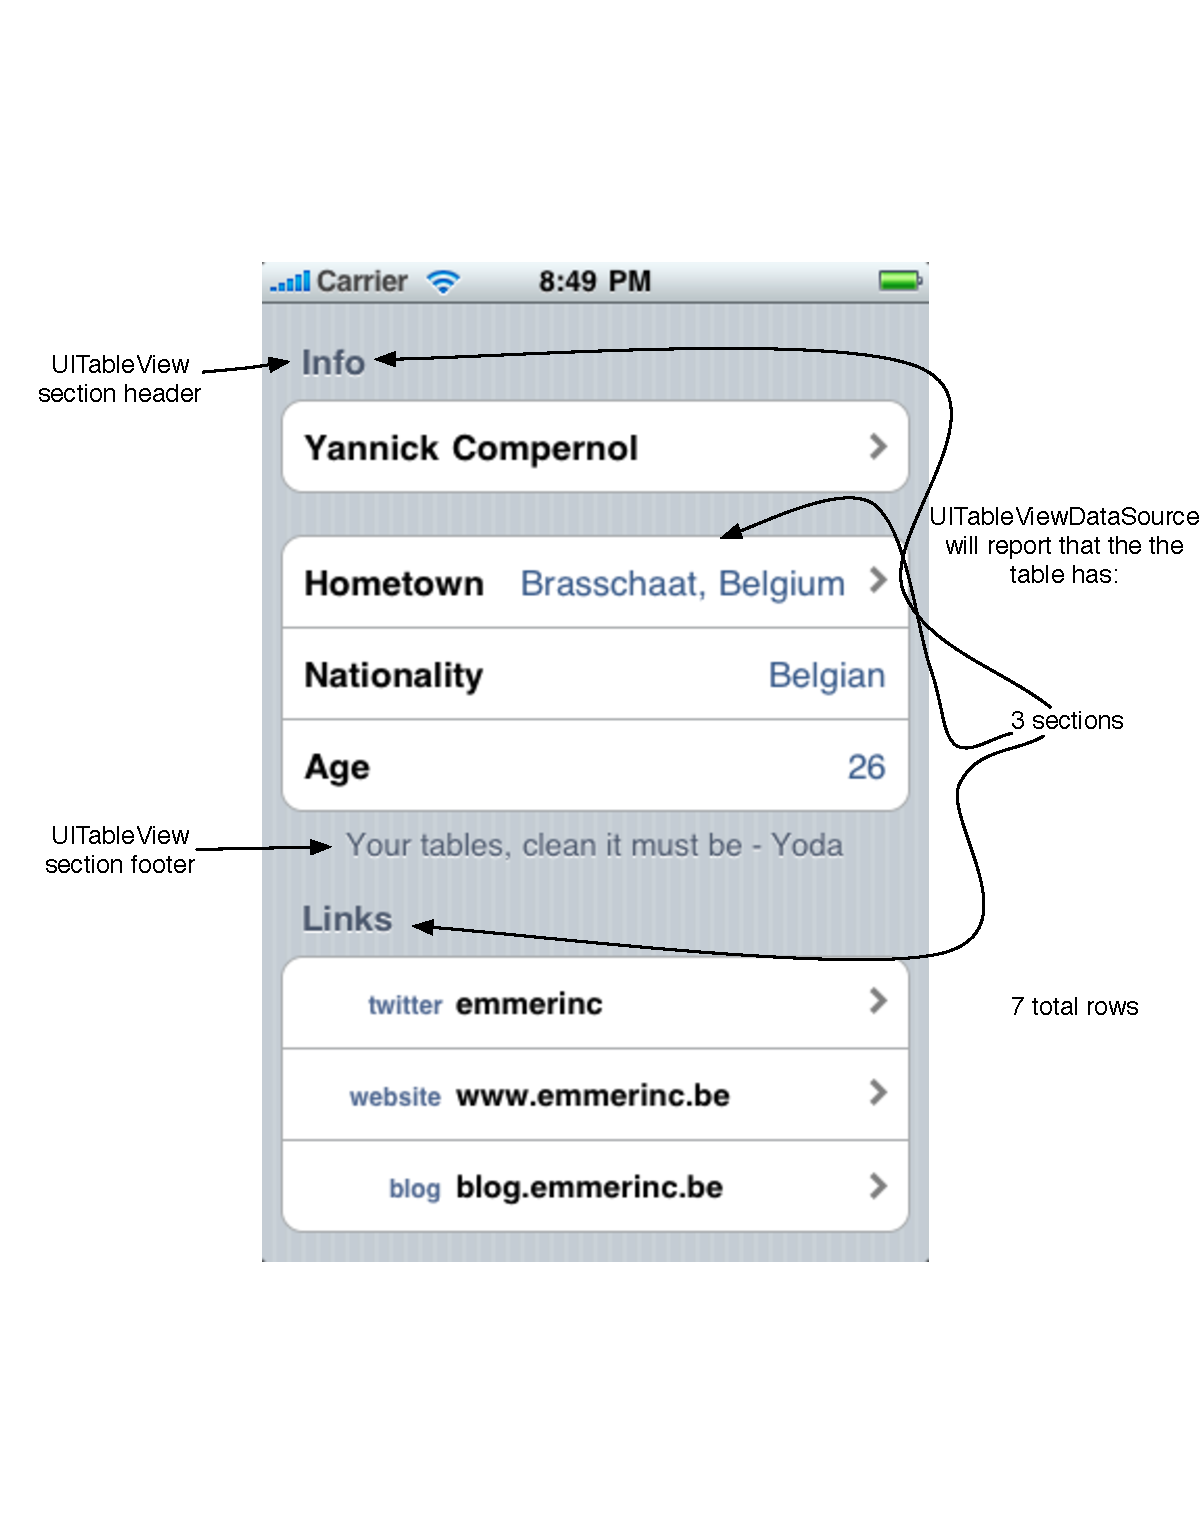
\includegraphics[scale=0.3]{UIViewExample5.pdf}
              
  \caption{UITableView example}
  \end{center}
  \end{figure}

\end{frame}

    
\begin{frame}[fragile]
  \frametitle{Lab 3}
  Add a UITableViewController to the project

\end{frame}

\begin{frame}[fragile]
  \frametitle{Lab 3}
  Add an NSArray containing names from the class to the controller

\end{frame}

\begin{frame}[fragile]
  \frametitle{Lab 3}
  Change the Interface builder reference to the UITableViewController

\end{frame}

    
\begin{frame}[fragile]
  \frametitle{Modal view controllers}
  Not all view controllers fit within the "display in UINavigationController" or "display in UITabBarController" model.

\end{frame}

\begin{frame}[fragile]
  \frametitle{Modal view controllers}
  \begin{figure}[htb]
  \begin{center}
  
  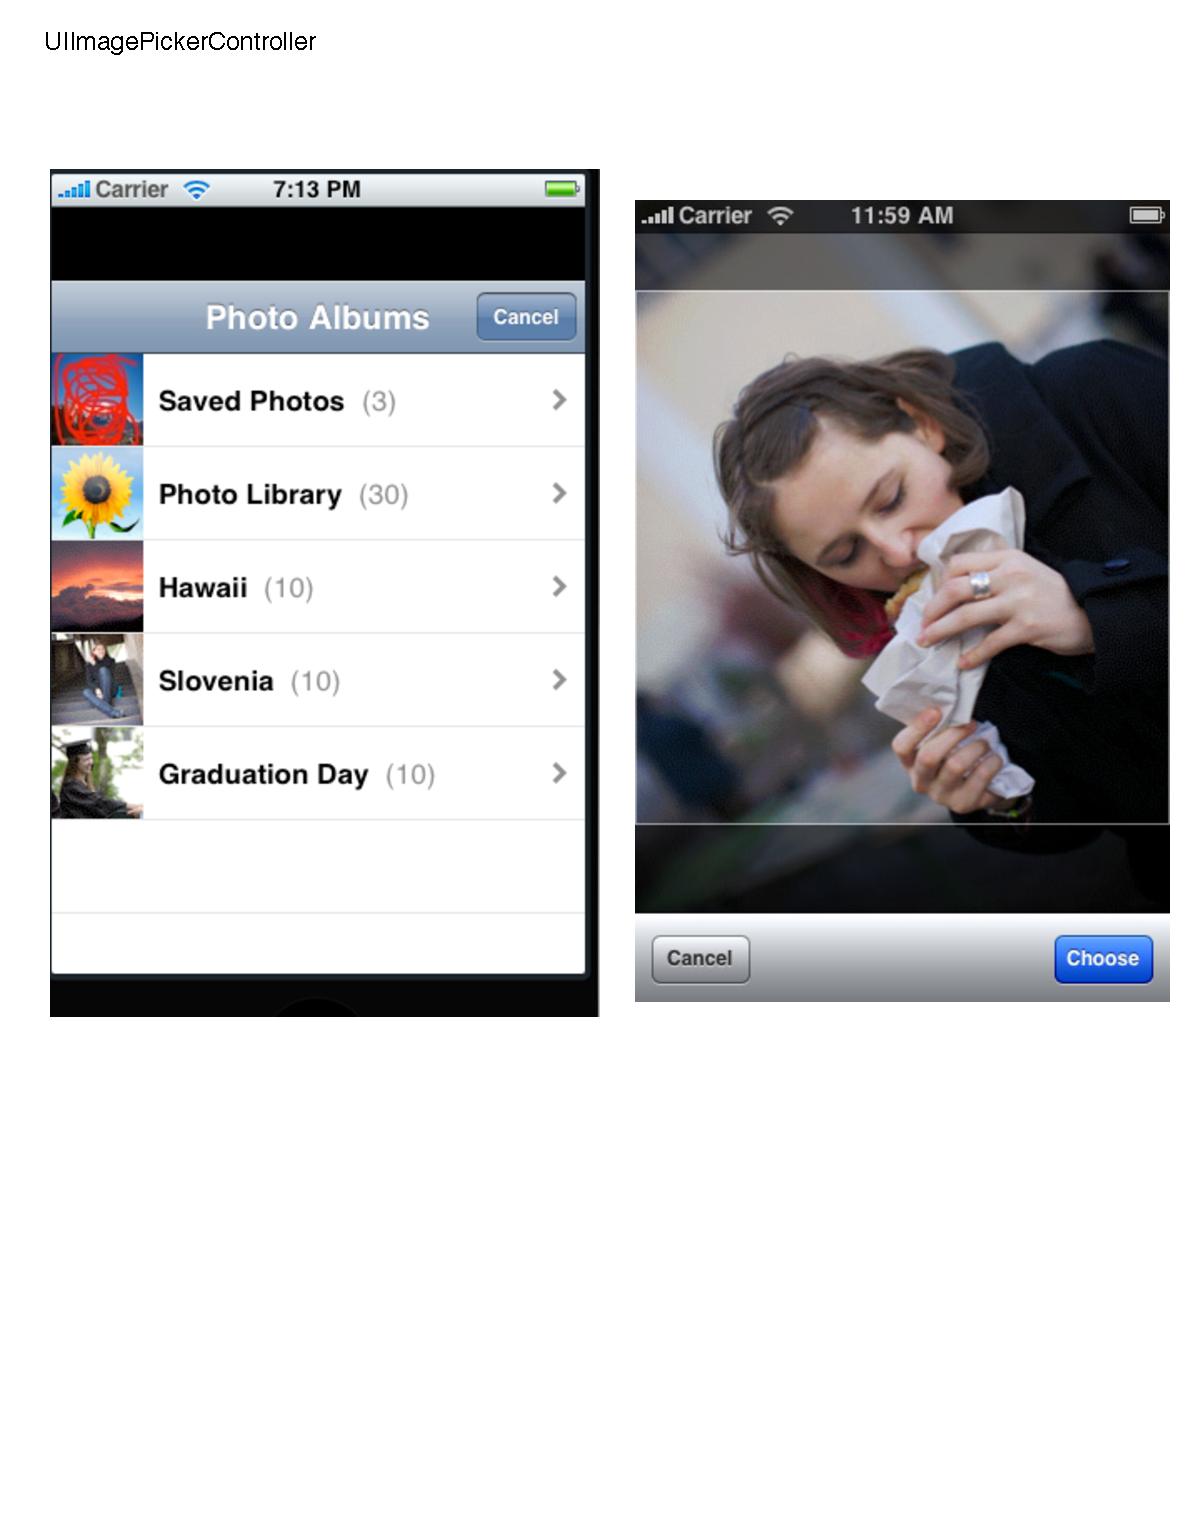
\includegraphics[scale=0.35]{UIViewExample6.pdf}
            
  \caption{UIImagePickerController}
  \end{center}
  \end{figure}

\end{frame}

\begin{frame}[fragile]
  \frametitle{Modal view controllers}
  \begin{figure}[htb]
  \begin{center}
  
  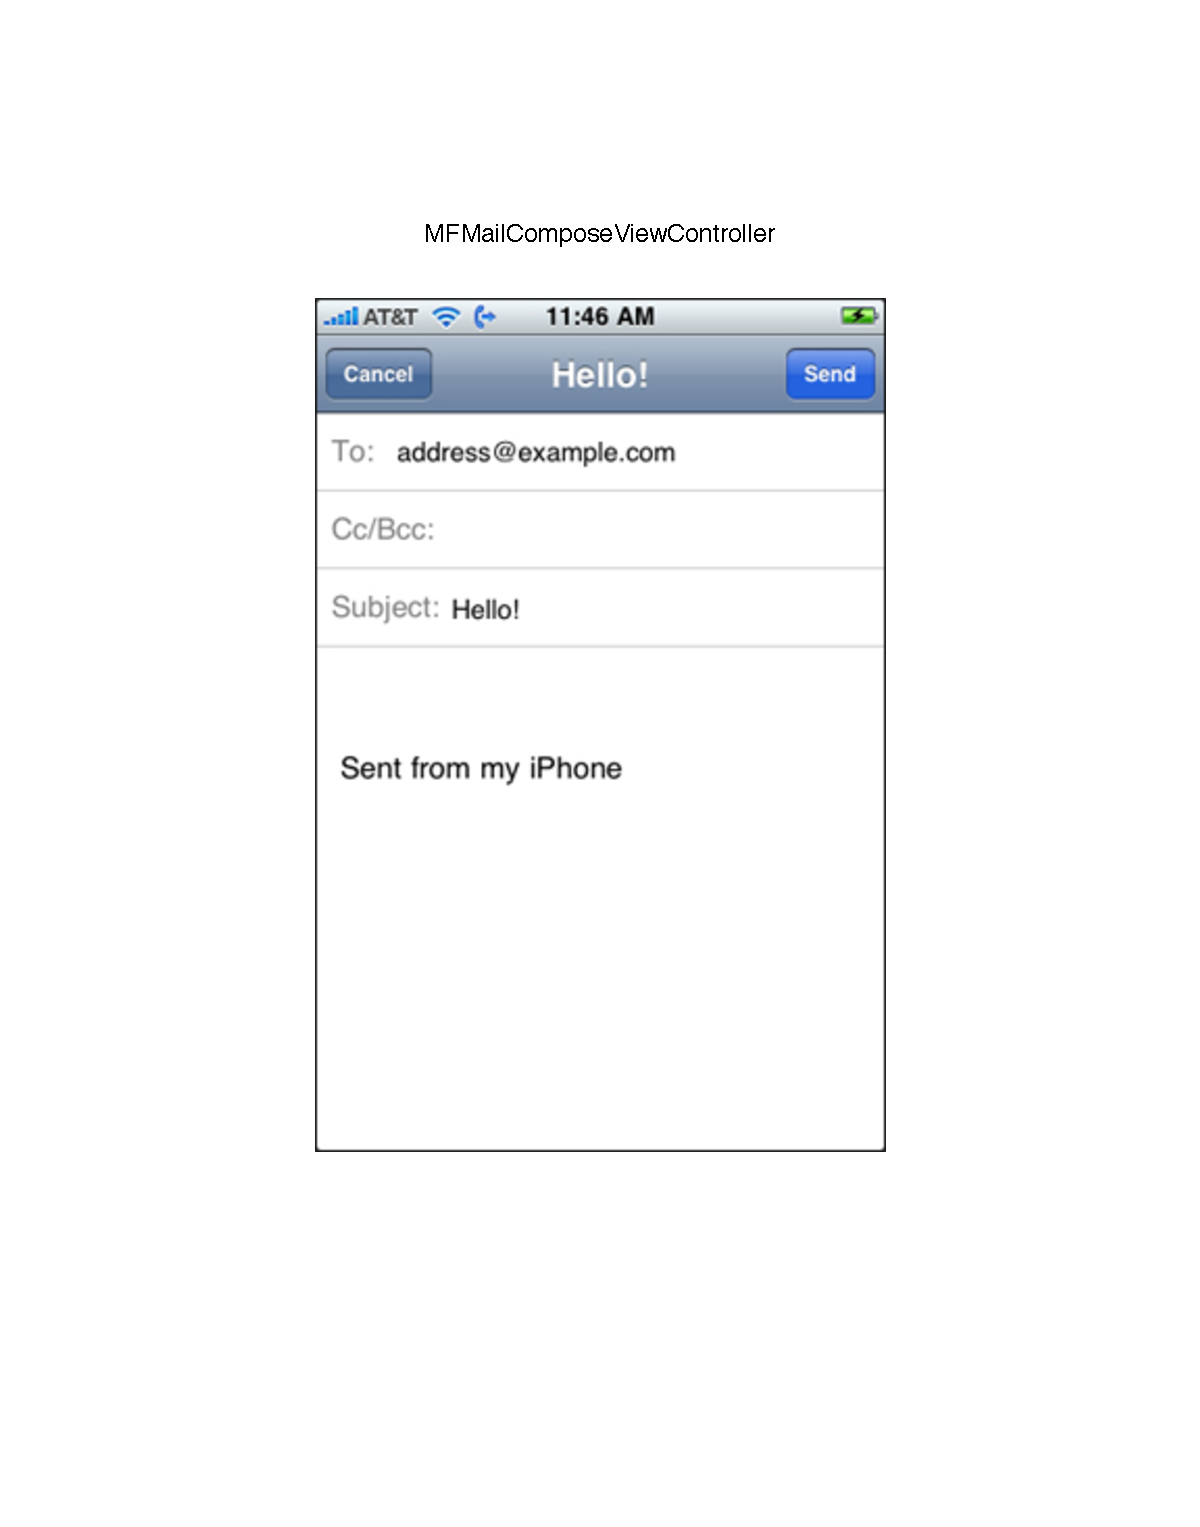
\includegraphics[scale=0.35]{UIViewExample7.pdf}
            
  \caption{MFMailComposeViewController}
  \end{center}
  \end{figure}

\end{frame}

\begin{frame}[fragile]
  \frametitle{Modal view controllers}
  You can present a view controller modally by using the presentModalViewController:animated: message
\begin{listing}[H]
    \begin{minted}[resetmargins=true,fontsize=\footnotesize]{objectivec}
  
  -(IBAction) buttonClicked:(id) sender {
    MyViewController * mvc = [[MyViewController alloc] 
                                   initWithNibName:@"TheNib"
                                   bundle:nil];
    [self presentModalViewController:mvc animated:YES];
    [mvc release];
  }
            
  \end{minted}
    \caption{Presenting a view controller modally}
    \label{listing:26}
  \end{listing}

\end{frame}

\begin{frame}[fragile]
  \frametitle{Modal view controllers}
  You can specify the transition style with which the view controller appears via the UIViewController message \begin{minted}[resetmargins=true,fontsize=\footnotesize]{objectivec}
  
  setModalTransitionStyle:(UIModalTransitionStyle)style
            
  \end{minted} 

\end{frame}

    

% END SECTION iPhone App Layout Conventions
   
  

  
    
% BEGIN SECTION XCode and Interface Builder
\section{XCode and Interface Builder}
\begin{frame}[fragile]
  \frametitle{XCode and Interface Builder}
  5. XCode and Interface Builder
\end{frame}


    
\begin{frame}[fragile]
  \frametitle{Capabilities}
  XCode and Interface Builder combined provide a development, debugging and interface development tool for you to develop your iPhone apps.  It can integrate with SVN, CVS or Perforce ( and soon, Git! ), it can run automated tests on your code, provide inline documentation assist, code completion and a lot more. It also provides a developer level interface to all the devices you will be debugging your code on; you can manage devices and device profiles through XCode as necessary.

\end{frame}

    
\begin{frame}[fragile]
  \frametitle{Creating an app}
  XCode provides a number of application templates for starting an app.  Most basic types of applications can get a fast start by using one of these app templates. \begin{figure}[htb]
  \begin{center}
  
  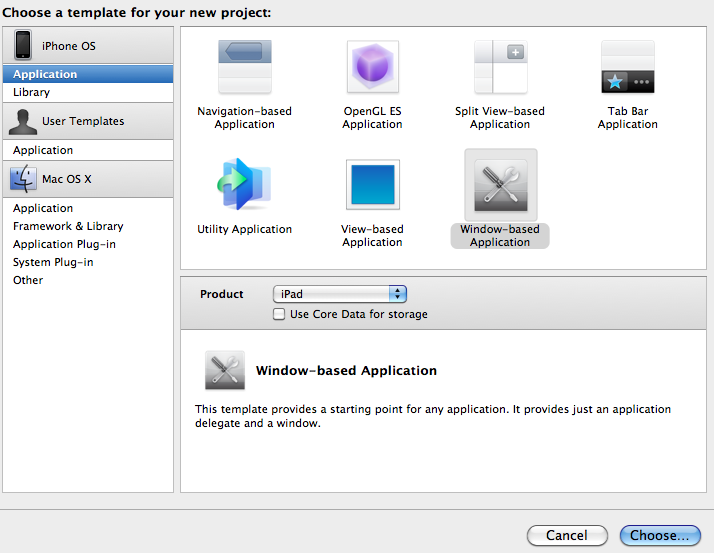
\includegraphics[scale=0.35]{ProjectCreator.png}
              
  \caption{XCode New Project window}
  \end{center}
  \end{figure}

\end{frame}

\begin{frame}[fragile]
  \frametitle{Creating an app}
  Once you've selected the type of app you want to create, your project will be created with an application delegate and usually at least one view controller that will manage what goes on the screen.  It will also have a .xib file for your application, and for each view controller in the app, that is used by Interface Builder to layout the screen contents. \begin{figure}[htb]
  \begin{center}
  
  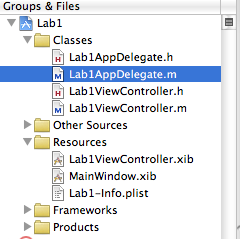
\includegraphics[scale=0.75]{ProjectFileList.png}
              
  \caption{New Project File List}
  \end{center}
  \end{figure}
\begin{block}{The application delegate - UIApplicationDelegate}
  
  The application delegate ( UIApplicationDelegate protocol ) is the class which will respond to overall application lifecycle events,
  like when your application has started, resumed from suspension, or is about to shut down. 
              
  \end{block}

\end{frame}

\begin{frame}[fragile]
  \frametitle{Creating an app}
  Double clicking on a .xib file will open it in Interface Builder, where you can drag components from the Interface Builder toolbox into the view.  You can easily change the orientation of objects.

\end{frame}

    
\begin{frame}[fragile]
  \frametitle{Documentation usage}
  \highlighton{Help - Developer Documentation} is an invaluable resource for researching Cocoa internals.

\end{frame}

    
\begin{frame}[fragile]
  \frametitle{Protips!}
  Learn hotkeys! ( CMD+SHIFT+D  and CMD+0 will buy you hours )

\end{frame}

\begin{frame}[fragile]
  \frametitle{Protips!}
  Make XCode fit you ( Single window interface, XCode themes, application templates )

\end{frame}

\begin{frame}[fragile]
  \frametitle{Protips!}
  XCode plugins ( Code Pilot \url{http://mac.brothersoft.com/code-pilot-for-xcode.html}, Accessorizer \url{http://www.kevincallahan.org/software/accessorizer.html} )

\end{frame}

    

% END SECTION XCode and Interface Builder
   
  

  
% BEGIN SECTION Questions
\section{Questions}
\begin{frame}[fragile]
  \frametitle{Questions}
  
\end{frame}

% END SECTION Questions

  


\bibliography{slides}{}
\bibliographystyle{plain}

\end{document}
